% Generated by render_manuscript_artifacts.py from campaign root code/output_overhaul_20260601
\begin{table}[t]
\centering
\small
\caption{Registry-defined public candidate evaluation campaign.}
\label{tab:candidate-campaign}
\resizebox{\textwidth}{!}{%
\begin{tabular}{lllllllll}
\toprule
Candidate & status & SR & HAC p+ & Boot p+ & RW p & Perm p & Net SR & Pass 5\% \\
\midrule
french\_momentum\_deciles\_daily\_rank & Available & 0.447 & 7.54e-05 & 2.00e-04 & 2.00e-04 & 1.000 & 0.447 & no \\
french\_momentum\_deciles\_daily\_wml & Available & 0.497 & 5.53e-06 & 2.00e-04 & 2.00e-04 & 1.00e-04 & 0.497 & yes \\
french\_size\_bm\_daily\_dynamic\_momentum & Available & 0.036 & 0.445 & 0.458 & 0.516 & 0.947 & -0.072 & no \\
stooq\_fixed\_etf\_daily\_dynamic\_momentum & Data unavailable &  &  &  &  &  &  & no \\
aqr\_bab\_equity\_factors\_daily & Available & 0.741 & 3.08e-13 & 2.00e-04 & 2.00e-04 &  & 0.741 & no \\
aqr\_qmj\_factors\_daily & Available & 0.536 & 2.26e-05 & 2.00e-04 & 2.00e-04 &  & 0.536 & no \\
aqr\_hml\_devil\_factors\_daily & Available & 0.336 & 0.004 & 0.002 & 0.002 &  & 0.336 & no \\
aqr\_value\_momentum\_everywhere\_monthly & Available & 2.623 & 1.62e-04 & 2.00e-04 & 2.00e-04 &  & 2.623 & no \\
\bottomrule
\end{tabular}%
}
\end{table}

\begin{table}[t]
\centering
\small
\caption{Canonical French momentum benchmark validation.}
\label{tab:momentum-benchmark}
\resizebox{\textwidth}{!}{%
\begin{tabular}{llllllll}
\toprule
Candidate & thr & n & start & end & panel SR & direct WML SR & scale \\
\midrule
french\_momentum\_deciles\_daily\_wml & 0.900 & 26131 & 1926-11-04 & 2026-04-30 & 0.497 & 0.497 & 0.500 \\
\bottomrule
\end{tabular}%
}
\end{table}

\begin{table}[t]
\centering
\small
\caption{Sampling-boundary design-effect diagnostics.}
\label{tab:row-boundary}
\resizebox{\textwidth}{!}{%
\begin{tabular}{lllllllllllll}
\toprule
Candidate & status & thr & rows & dates & avg names & rho & SE infl. & row t & HAC z & row p+ & HAC p+ & RW p \\
\midrule
aqr\_bab\_equity\_factors\_daily & not\_applicable\_single\_series & 0.000 & 25281 & 25281 & 1.000 &  &  &  &  &  &  & 2.00e-04 \\
aqr\_hml\_devil\_factors\_daily & not\_applicable\_single\_series & 0.000 & 26590 & 26590 & 1.000 &  &  &  &  &  &  & 0.002 \\
aqr\_qmj\_factors\_daily & not\_applicable\_single\_series & 0.000 & 17681 & 17681 & 1.000 &  &  &  &  &  &  & 2.00e-04 \\
aqr\_value\_momentum\_everywhere\_monthly & not\_applicable\_single\_series & 0.000 & 651 & 651 & 1.000 &  &  &  &  &  &  & 2.00e-04 \\
french\_momentum\_deciles\_daily\_rank & Available & 0.700 & 104524 & 26131 & 4.000 & -0.138 & 0.766 & 3.584 & 3.790 & 1.70e-04 & 7.54e-05 & 2.00e-04 \\
french\_momentum\_deciles\_daily\_wml & Available & 0.900 & 52262 & 26131 & 2.000 & -0.583 & 0.646 & 3.299 & 4.395 & 4.85e-04 & 5.53e-06 & 2.00e-04 \\
french\_size\_bm\_daily\_dynamic\_momentum & Available & 0.500 & 45201 & 3477 & 13.000 & 0.667 & 3.000 & 0.664 & 0.222 & 0.253 & 0.412 & 0.516 \\
\bottomrule
\end{tabular}%
}
\end{table}

\begin{table}[t]
\centering
\small
\caption{Dependence audit summary for panel candidates.}
\label{tab:phantom-audit}
\resizebox{\textwidth}{!}{%
\begin{tabular}{lllllll}
\toprule
Candidate & Row p+ & UVIF & EIR & Audit p+ & Net SR & Status \\
\midrule
french\_momentum\_deciles\_daily\_rank & 1.70e-04 & 1.000 & 1.000 & 1.000 & 0.447 & Fails permutation gate \\
french\_momentum\_deciles\_daily\_wml & 4.85e-04 & 1.000 & 1.000 & 2.00e-04 & 0.497 & Passes composite gate \\
french\_size\_bm\_daily\_dynamic\_momentum & 0.253 & 9.002 & 0.111 & 0.947 & -0.072 & Fails cost gate \\
\bottomrule
\end{tabular}%
}
\par\footnotesize\emph{Note:} EIR is a diagnostic approximation and is not used as a rejection rule.
\end{table}

\begin{table}[t]
\centering
\small
\caption{Horizon-effect audit for the dynamic Size/BM momentum panel.}
\label{tab:horizon-effect}
\resizebox{\textwidth}{!}{%
\begin{tabular}{llllllllll}
\toprule
L & thr & dates & avg names & gross SR & net SR 5bps & turnover & UVIF SR & serial UVIF & HAC p+ \\
\midrule
1 & 0.500 & 3497 & 12.913 & 0.073 & -0.394 & 0.733 & 11.498 & 0.891 & 0.386 \\
5 & 0.500 & 3493 & 13.000 & -0.312 & -0.528 & 0.339 & 12.880 & 0.990 & 0.878 \\
21 & 0.500 & 3477 & 13.000 & 0.058 & -0.050 & 0.169 & 12.121 & 0.933 & 0.412 \\
\bottomrule
\end{tabular}%
}
\end{table}

\begin{table}[t]
\centering
\small
\caption{Primary-threshold dependence-aware Sharpe inference.}
\label{tab:empirical-inference}
\resizebox{\textwidth}{!}{%
\begin{tabular}{lllllllll}
\toprule
Candidate & thr & Method & SR & SE & CI low & CI high & p+ & n \\
\midrule
aqr\_bab\_equity\_factors\_daily & 0.000 & block & 0.741 & 0.106 & 0.533 & 0.951 & 2.00e-04 & 25281 \\
aqr\_bab\_equity\_factors\_daily & 0.000 & HAC & 0.741 & 0.103 & 0.540 & 0.943 & 3.08e-13 & 25281 \\
aqr\_bab\_equity\_factors\_daily & 0.000 & prewhite & 0.741 & 0.104 & 0.538 & 0.945 & 4.38e-13 & 25281 \\
aqr\_hml\_devil\_factors\_daily & 0.000 & block & 0.336 & 0.114 & 0.105 & 0.552 & 0.002 & 26590 \\
aqr\_hml\_devil\_factors\_daily & 0.000 & HAC & 0.336 & 0.126 & 0.089 & 0.583 & 0.004 & 26590 \\
aqr\_hml\_devil\_factors\_daily & 0.000 & prewhite & 0.336 & 0.111 & 0.119 & 0.553 & 0.001 & 26590 \\
aqr\_qmj\_factors\_daily & 0.000 & block & 0.536 & 0.133 & 0.276 & 0.795 & 2.00e-04 & 17681 \\
aqr\_qmj\_factors\_daily & 0.000 & HAC & 0.536 & 0.131 & 0.279 & 0.794 & 2.26e-05 & 17681 \\
aqr\_qmj\_factors\_daily & 0.000 & prewhite & 0.536 & 0.128 & 0.285 & 0.787 & 1.40e-05 & 17681 \\
aqr\_value\_momentum\_everywhere\_monthly & 0.000 & block & 2.623 & 0.716 & 1.230 & 4.041 & 2.00e-04 & 651 \\
aqr\_value\_momentum\_everywhere\_monthly & 0.000 & HAC & 2.625 & 0.730 & 1.194 & 4.056 & 1.62e-04 & 651 \\
aqr\_value\_momentum\_everywhere\_monthly & 0.000 & prewhite & 2.625 & 0.723 & 1.207 & 4.043 & 1.42e-04 & 651 \\
french\_momentum\_deciles\_daily\_rank & 0.700 & block & 0.447 & 0.114 & 0.222 & 0.667 & 2.00e-04 & 26131 \\
french\_momentum\_deciles\_daily\_rank & 0.700 & HAC & 0.447 & 0.118 & 0.216 & 0.679 & 7.54e-05 & 26131 \\
french\_momentum\_deciles\_daily\_rank & 0.700 & prewhite & 0.447 & 0.114 & 0.224 & 0.670 & 4.18e-05 & 26131 \\
french\_momentum\_deciles\_daily\_wml & 0.900 & block & 0.497 & 0.111 & 0.275 & 0.708 & 2.00e-04 & 26131 \\
french\_momentum\_deciles\_daily\_wml & 0.900 & HAC & 0.497 & 0.113 & 0.275 & 0.718 & 5.53e-06 & 26131 \\
french\_momentum\_deciles\_daily\_wml & 0.900 & prewhite & 0.497 & 0.111 & 0.279 & 0.715 & 3.99e-06 & 26131 \\
french\_size\_bm\_daily\_dynamic\_momentum & 0.500 & block & 0.036 & 0.261 & -0.487 & 0.530 & 0.458 & 3477 \\
french\_size\_bm\_daily\_dynamic\_momentum & 0.500 & HAC & 0.036 & 0.260 & -0.473 & 0.544 & 0.445 & 3477 \\
\bottomrule
\end{tabular}%
}
\end{table}

\begin{table}[t]
\centering
\small
\caption{Same-date signal-permutation diagnostics for panel candidates.}
\label{tab:permutation}
\resizebox{\textwidth}{!}{%
\begin{tabular}{lllllll}
\toprule
Candidate & thr & obs SR & null mean & null sd & p+ & perms \\
\midrule
french\_momentum\_deciles\_daily\_rank & 0.000 & 0.395 & 0.410 & 0.039 & 0.646 & 10000 \\
french\_momentum\_deciles\_daily\_rank & 0.300 & 0.419 & 0.434 & 0.024 & 0.733 & 10000 \\
french\_momentum\_deciles\_daily\_rank & 0.500 & 0.419 & 0.434 & 0.024 & 0.733 & 10000 \\
french\_momentum\_deciles\_daily\_rank & 0.700 & 0.447 & 0.447 & 1.11e-16 & 1.000 & 10000 \\
french\_momentum\_deciles\_daily\_rank & 0.900 & 0.497 & 0.404 & 0.042 & 0.015 & 10000 \\
french\_momentum\_deciles\_daily\_wml & 0.900 & 0.497 & -0.001 & 0.098 & 1.00e-04 & 10000 \\
french\_size\_bm\_daily\_dynamic\_momentum & 0.000 & 0.011 & 0.052 & 0.017 & 0.993 & 10000 \\
french\_size\_bm\_daily\_dynamic\_momentum & 0.300 & 0.010 & 0.072 & 0.023 & 0.996 & 10000 \\
french\_size\_bm\_daily\_dynamic\_momentum & 0.500 & 0.036 & 0.083 & 0.029 & 0.947 & 10000 \\
french\_size\_bm\_daily\_dynamic\_momentum & 0.700 & 0.061 & 0.112 & 0.040 & 0.893 & 10000 \\
french\_size\_bm\_daily\_dynamic\_momentum & 0.900 & 0.025 & 0.098 & 0.069 & 0.855 & 10000 \\
\bottomrule
\end{tabular}%
}
\end{table}

\begin{table}[t]
\centering
\small
\caption{HAC bandwidth, prewhitening, and fixed-b robustness diagnostics.}
\label{tab:hac-robustness}
\resizebox{\textwidth}{!}{%
\begin{tabular}{lllll}
\toprule
Candidate & Diagnostic & SR & SE & p+ \\
\midrule
aqr\_bab\_equity\_factors\_daily & HAC K=auto & 0.741 & 0.103 & 3.08e-13 \\
aqr\_bab\_equity\_factors\_daily & HAC K=21 & 0.741 & 0.119 & 2.04e-10 \\
aqr\_bab\_equity\_factors\_daily & HAC K=63 & 0.741 & 0.130 & 6.06e-09 \\
aqr\_bab\_equity\_factors\_daily & prewhite & 0.741 & 0.104 & 4.38e-13 \\
aqr\_bab\_equity\_factors\_daily & fixed-b 0.1 & 0.741 & 0.166 & 0.002 \\
aqr\_hml\_devil\_factors\_daily & HAC K=auto & 0.336 & 0.126 & 0.004 \\
aqr\_hml\_devil\_factors\_daily & HAC K=21 & 0.336 & 0.128 & 0.004 \\
aqr\_hml\_devil\_factors\_daily & HAC K=63 & 0.336 & 0.137 & 0.007 \\
aqr\_hml\_devil\_factors\_daily & prewhite & 0.336 & 0.111 & 0.001 \\
aqr\_hml\_devil\_factors\_daily & fixed-b 0.1 & 0.336 & 0.110 & 0.004 \\
aqr\_qmj\_factors\_daily & HAC K=auto & 0.536 & 0.131 & 2.26e-05 \\
aqr\_qmj\_factors\_daily & HAC K=21 & 0.536 & 0.140 & 6.33e-05 \\
aqr\_qmj\_factors\_daily & HAC K=63 & 0.536 & 0.147 & 1.32e-04 \\
aqr\_qmj\_factors\_daily & prewhite & 0.536 & 0.128 & 1.40e-05 \\
aqr\_qmj\_factors\_daily & fixed-b 0.1 & 0.536 & 0.151 & 0.002 \\
aqr\_value\_momentum\_everywhere\_monthly & HAC K=auto & 2.625 & 0.730 & 1.62e-04 \\
aqr\_value\_momentum\_everywhere\_monthly & HAC K=21 & 2.625 & 0.712 & 1.14e-04 \\
aqr\_value\_momentum\_everywhere\_monthly & HAC K=63 & 2.625 & 0.659 & 3.41e-05 \\
aqr\_value\_momentum\_everywhere\_monthly & prewhite & 2.625 & 0.723 & 1.42e-04 \\
aqr\_value\_momentum\_everywhere\_monthly & fixed-b 0.1 & 2.625 & 0.656 & 0.004 \\
french\_momentum\_deciles\_daily\_rank & HAC K=auto & 0.447 & 0.118 & 7.54e-05 \\
french\_momentum\_deciles\_daily\_rank & HAC K=21 & 0.447 & 0.120 & 9.94e-05 \\
french\_momentum\_deciles\_daily\_rank & HAC K=63 & 0.447 & 0.122 & 1.21e-04 \\
french\_momentum\_deciles\_daily\_rank & prewhite & 0.447 & 0.114 & 4.18e-05 \\
french\_momentum\_deciles\_daily\_rank & fixed-b 0.1 & 0.447 & 0.143 & 0.004 \\
french\_momentum\_deciles\_daily\_wml & HAC K=auto & 0.497 & 0.113 & 5.53e-06 \\
french\_momentum\_deciles\_daily\_wml & HAC K=21 & 0.497 & 0.116 & 9.62e-06 \\
french\_momentum\_deciles\_daily\_wml & HAC K=63 & 0.497 & 0.117 & 1.01e-05 \\
french\_momentum\_deciles\_daily\_wml & prewhite & 0.497 & 0.111 & 3.99e-06 \\
french\_momentum\_deciles\_daily\_wml & fixed-b 0.1 & 0.497 & 0.147 & 0.002 \\
\bottomrule
\end{tabular}%
}
\end{table}

\begin{table}[t]
\centering
\small
\caption{Composite gate sensitivity by alpha threshold.}
\label{tab:gate-sensitivity}
\resizebox{\textwidth}{!}{%
\begin{tabular}{lll}
\toprule
alpha & candidates & passes \\
\midrule
0.010 & 8 & 1 \\
0.050 & 8 & 1 \\
\bottomrule
\end{tabular}%
}
\end{table}

\begin{table}[t]
\centering
\small
\caption{Holdout and subperiod Sharpe diagnostics.}
\label{tab:holdout-subperiods}
\resizebox{\textwidth}{!}{%
\begin{tabular}{llll}
\toprule
Candidate & window & SR & n \\
\midrule
aqr\_bab\_equity\_factors\_daily & train\_70pct & 0.887 & 17696 \\
aqr\_bab\_equity\_factors\_daily & holdout\_30pct & 0.531 & 7585 \\
aqr\_bab\_equity\_factors\_daily & quarter\_min & 0.280 & 6320 \\
aqr\_bab\_equity\_factors\_daily & quarter\_max & 1.270 & 6320 \\
aqr\_hml\_devil\_factors\_daily & train\_70pct & 0.465 & 18613 \\
aqr\_hml\_devil\_factors\_daily & holdout\_30pct & 0.120 & 7977 \\
aqr\_hml\_devil\_factors\_daily & quarter\_min & 0.273 & 6647 \\
aqr\_hml\_devil\_factors\_daily & quarter\_max & 0.445 & 6647 \\
aqr\_qmj\_factors\_daily & train\_70pct & 0.794 & 12376 \\
aqr\_qmj\_factors\_daily & holdout\_30pct & 0.305 & 5305 \\
aqr\_qmj\_factors\_daily & quarter\_min & 0.174 & 4421 \\
aqr\_qmj\_factors\_daily & quarter\_max & 1.083 & 4420 \\
aqr\_value\_momentum\_everywhere\_monthly & train\_70pct & 2.867 & 455 \\
aqr\_value\_momentum\_everywhere\_monthly & holdout\_30pct & 1.974 & 196 \\
aqr\_value\_momentum\_everywhere\_monthly & quarter\_min & 1.707 & 163 \\
aqr\_value\_momentum\_everywhere\_monthly & quarter\_max & 4.313 & 163 \\
french\_momentum\_deciles\_daily\_rank & train\_70pct & 0.615 & 18292 \\
french\_momentum\_deciles\_daily\_rank & holdout\_30pct & 0.229 & 7839 \\
french\_momentum\_deciles\_daily\_rank & quarter\_min & 0.171 & 6532 \\
french\_momentum\_deciles\_daily\_rank & quarter\_max & 1.280 & 6533 \\
french\_momentum\_deciles\_daily\_wml & train\_70pct & 0.641 & 18292 \\
french\_momentum\_deciles\_daily\_wml & holdout\_30pct & 0.310 & 7839 \\
french\_momentum\_deciles\_daily\_wml & quarter\_min & 0.224 & 6533 \\
french\_momentum\_deciles\_daily\_wml & quarter\_max & 1.370 & 6533 \\
french\_size\_bm\_daily\_dynamic\_momentum & train\_70pct & 0.050 & 2428 \\
french\_size\_bm\_daily\_dynamic\_momentum & holdout\_30pct & 0.005 & 1049 \\
french\_size\_bm\_daily\_dynamic\_momentum & quarter\_min & -0.657 & 853 \\
french\_size\_bm\_daily\_dynamic\_momentum & quarter\_max & 0.211 & 875 \\
\bottomrule
\end{tabular}%
}
\end{table}

\begin{table}[t]
\centering
\small
\caption{Turnover-scaled cost sensitivity and break-even cost.}
\label{tab:costs}
\resizebox{\textwidth}{!}{%
\begin{tabular}{llllll}
\toprule
Candidate & cost bps & turnover & gross SR & net SR & break-even bps \\
\midrule
aqr\_bab\_equity\_factors\_daily & 0 & 0.000 & 0.741 & 0.741 &  \\
aqr\_bab\_equity\_factors\_daily & 1 & 0.000 & 0.741 & 0.741 &  \\
aqr\_bab\_equity\_factors\_daily & 5 & 0.000 & 0.741 & 0.741 &  \\
aqr\_bab\_equity\_factors\_daily & 10 & 0.000 & 0.741 & 0.741 &  \\
aqr\_bab\_equity\_factors\_daily & 25 & 0.000 & 0.741 & 0.741 &  \\
aqr\_hml\_devil\_factors\_daily & 0 & 0.000 & 0.336 & 0.336 &  \\
aqr\_hml\_devil\_factors\_daily & 1 & 0.000 & 0.336 & 0.336 &  \\
aqr\_hml\_devil\_factors\_daily & 5 & 0.000 & 0.336 & 0.336 &  \\
aqr\_hml\_devil\_factors\_daily & 10 & 0.000 & 0.336 & 0.336 &  \\
aqr\_hml\_devil\_factors\_daily & 25 & 0.000 & 0.336 & 0.336 &  \\
aqr\_qmj\_factors\_daily & 0 & 0.000 & 0.536 & 0.536 &  \\
aqr\_qmj\_factors\_daily & 1 & 0.000 & 0.536 & 0.536 &  \\
aqr\_qmj\_factors\_daily & 5 & 0.000 & 0.536 & 0.536 &  \\
aqr\_qmj\_factors\_daily & 10 & 0.000 & 0.536 & 0.536 &  \\
aqr\_qmj\_factors\_daily & 25 & 0.000 & 0.536 & 0.536 &  \\
aqr\_value\_momentum\_everywhere\_monthly & 0 & 0.000 & 2.623 & 2.623 &  \\
aqr\_value\_momentum\_everywhere\_monthly & 1 & 0.000 & 2.623 & 2.623 &  \\
aqr\_value\_momentum\_everywhere\_monthly & 5 & 0.000 & 2.623 & 2.623 &  \\
aqr\_value\_momentum\_everywhere\_monthly & 10 & 0.000 & 2.623 & 2.623 &  \\
aqr\_value\_momentum\_everywhere\_monthly & 25 & 0.000 & 2.623 & 2.623 &  \\
french\_momentum\_deciles\_daily\_rank & 0 & 1.91e-05 & 0.447 & 0.447 & 85893.000 \\
french\_momentum\_deciles\_daily\_rank & 1 & 1.91e-05 & 0.447 & 0.447 & 85893.000 \\
french\_momentum\_deciles\_daily\_rank & 5 & 1.91e-05 & 0.447 & 0.447 & 85893.000 \\
french\_momentum\_deciles\_daily\_rank & 10 & 1.91e-05 & 0.447 & 0.447 & 85893.000 \\
french\_momentum\_deciles\_daily\_rank & 25 & 1.91e-05 & 0.447 & 0.447 & 85893.000 \\
french\_momentum\_deciles\_daily\_wml & 0 & 1.91e-05 & 0.497 & 0.497 & 122232.000 \\
french\_momentum\_deciles\_daily\_wml & 1 & 1.91e-05 & 0.497 & 0.497 & 122232.000 \\
french\_momentum\_deciles\_daily\_wml & 5 & 1.91e-05 & 0.497 & 0.497 & 122232.000 \\
french\_momentum\_deciles\_daily\_wml & 10 & 1.91e-05 & 0.497 & 0.497 & 122232.000 \\
french\_momentum\_deciles\_daily\_wml & 25 & 1.91e-05 & 0.497 & 0.497 & 122232.000 \\
french\_size\_bm\_daily\_dynamic\_momentum & 0 & 0.169 & 0.036 & 0.036 &  \\
french\_size\_bm\_daily\_dynamic\_momentum & 1 & 0.169 & 0.036 & 0.014 &  \\
french\_size\_bm\_daily\_dynamic\_momentum & 5 & 0.169 & 0.036 & -0.072 &  \\
french\_size\_bm\_daily\_dynamic\_momentum & 10 & 0.169 & 0.036 & -0.179 &  \\
french\_size\_bm\_daily\_dynamic\_momentum & 25 & 0.169 & 0.036 & -0.502 &  \\
\bottomrule
\end{tabular}%
}
\end{table}


\begin{figure}[t]
\centering
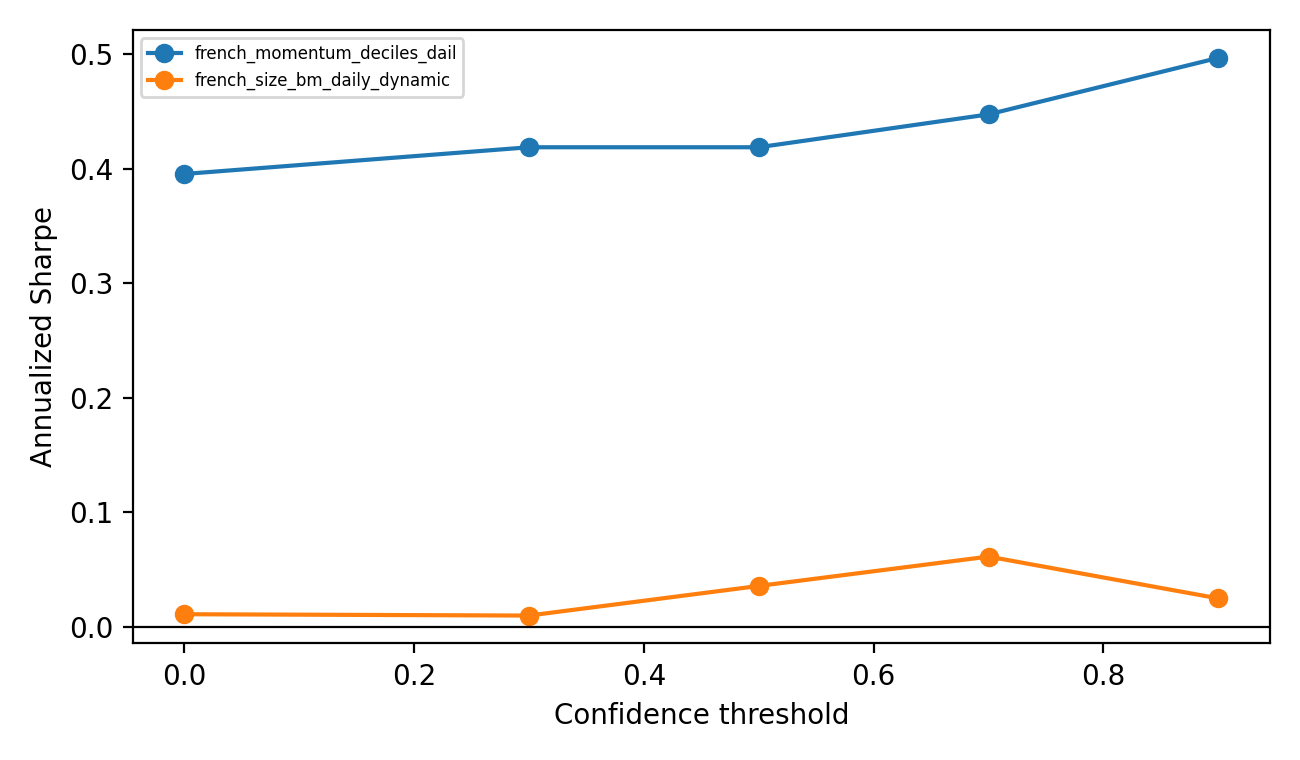
\includegraphics[width=0.82\textwidth]{generated_figures/threshold_profile.png}
\caption{Threshold profile for public candidate panels.}
\label{fig:threshold-profile}
\end{figure}

\begin{figure}[t]
\centering
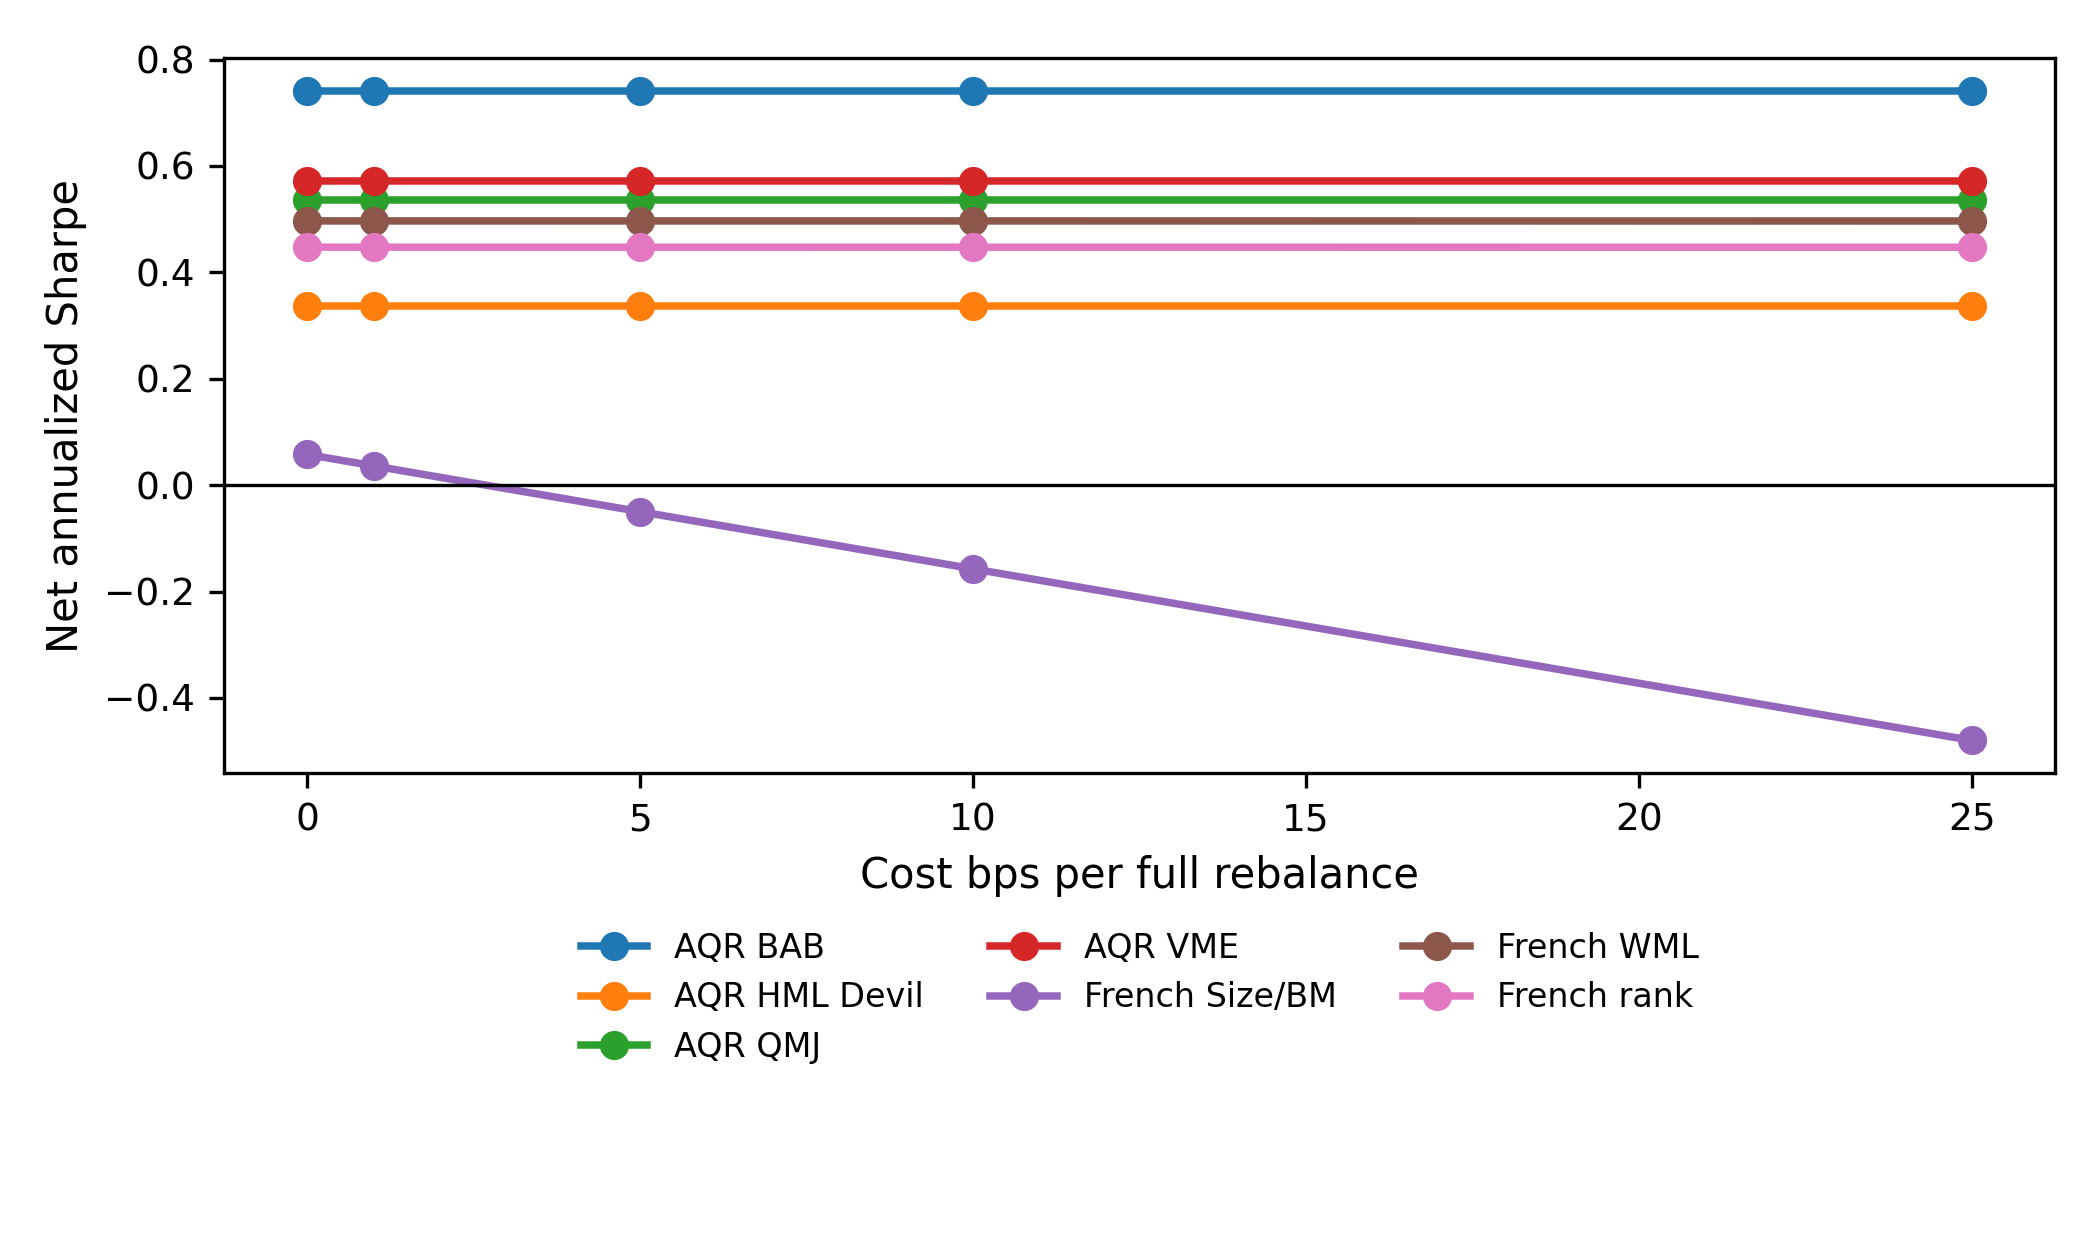
\includegraphics[width=0.82\textwidth]{generated_figures/cost_sensitivity.png}
\caption{Turnover-scaled cost sensitivity at primary candidate thresholds.}
\label{fig:cost-sensitivity}
\end{figure}
